%\subsection{Summary slides from the working sessions}

\begin{figure*}[p]
    \centering
    \fbox{
    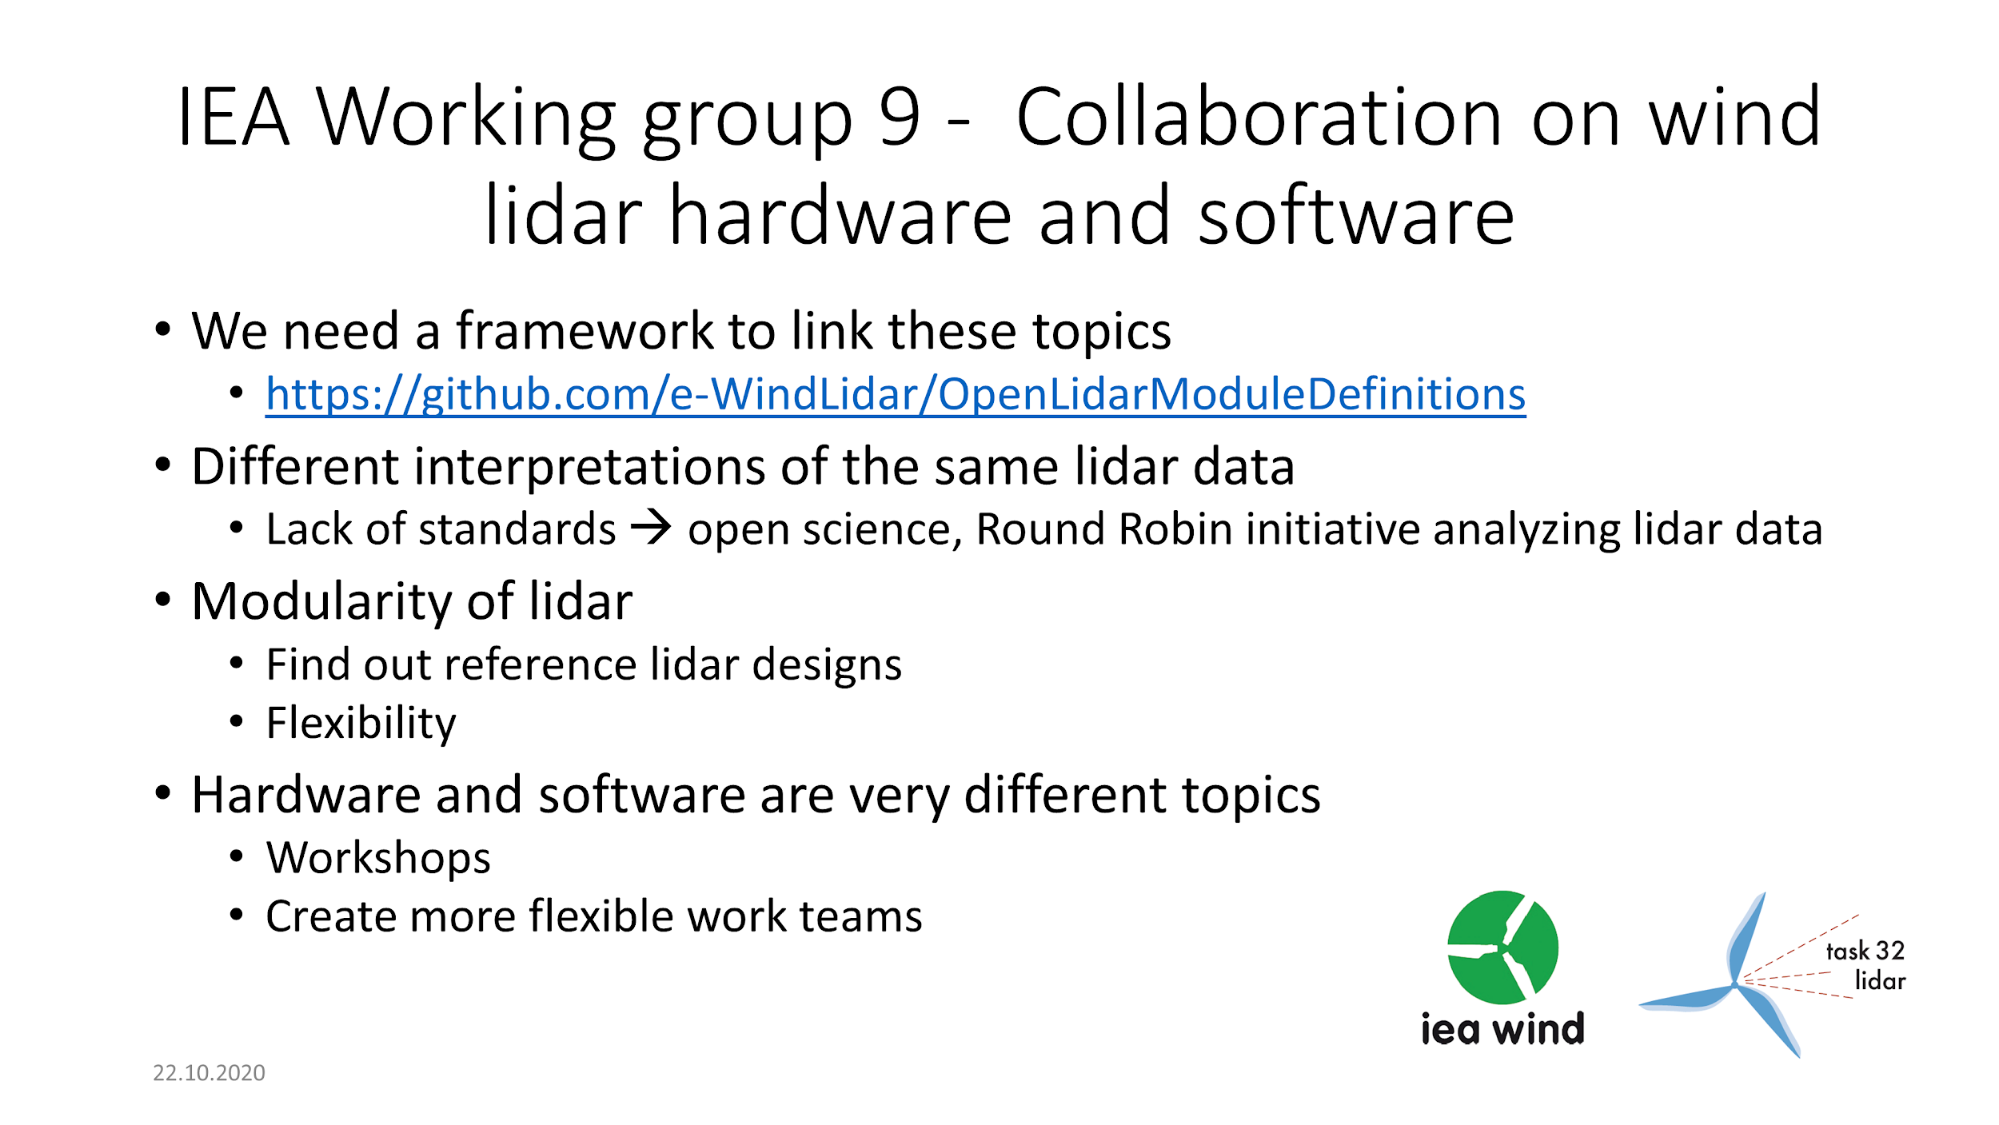
\includegraphics[width=0.85\textwidth]{figures/day3-collaboration-hardware-software.png}
    }
    \caption{Collaboration on wind lidar hardware and software}
    \label{fig:day3-collaboration-hardware-software}
\end{figure*}

\begin{figure*}[p]
    \centering
    \fbox{
    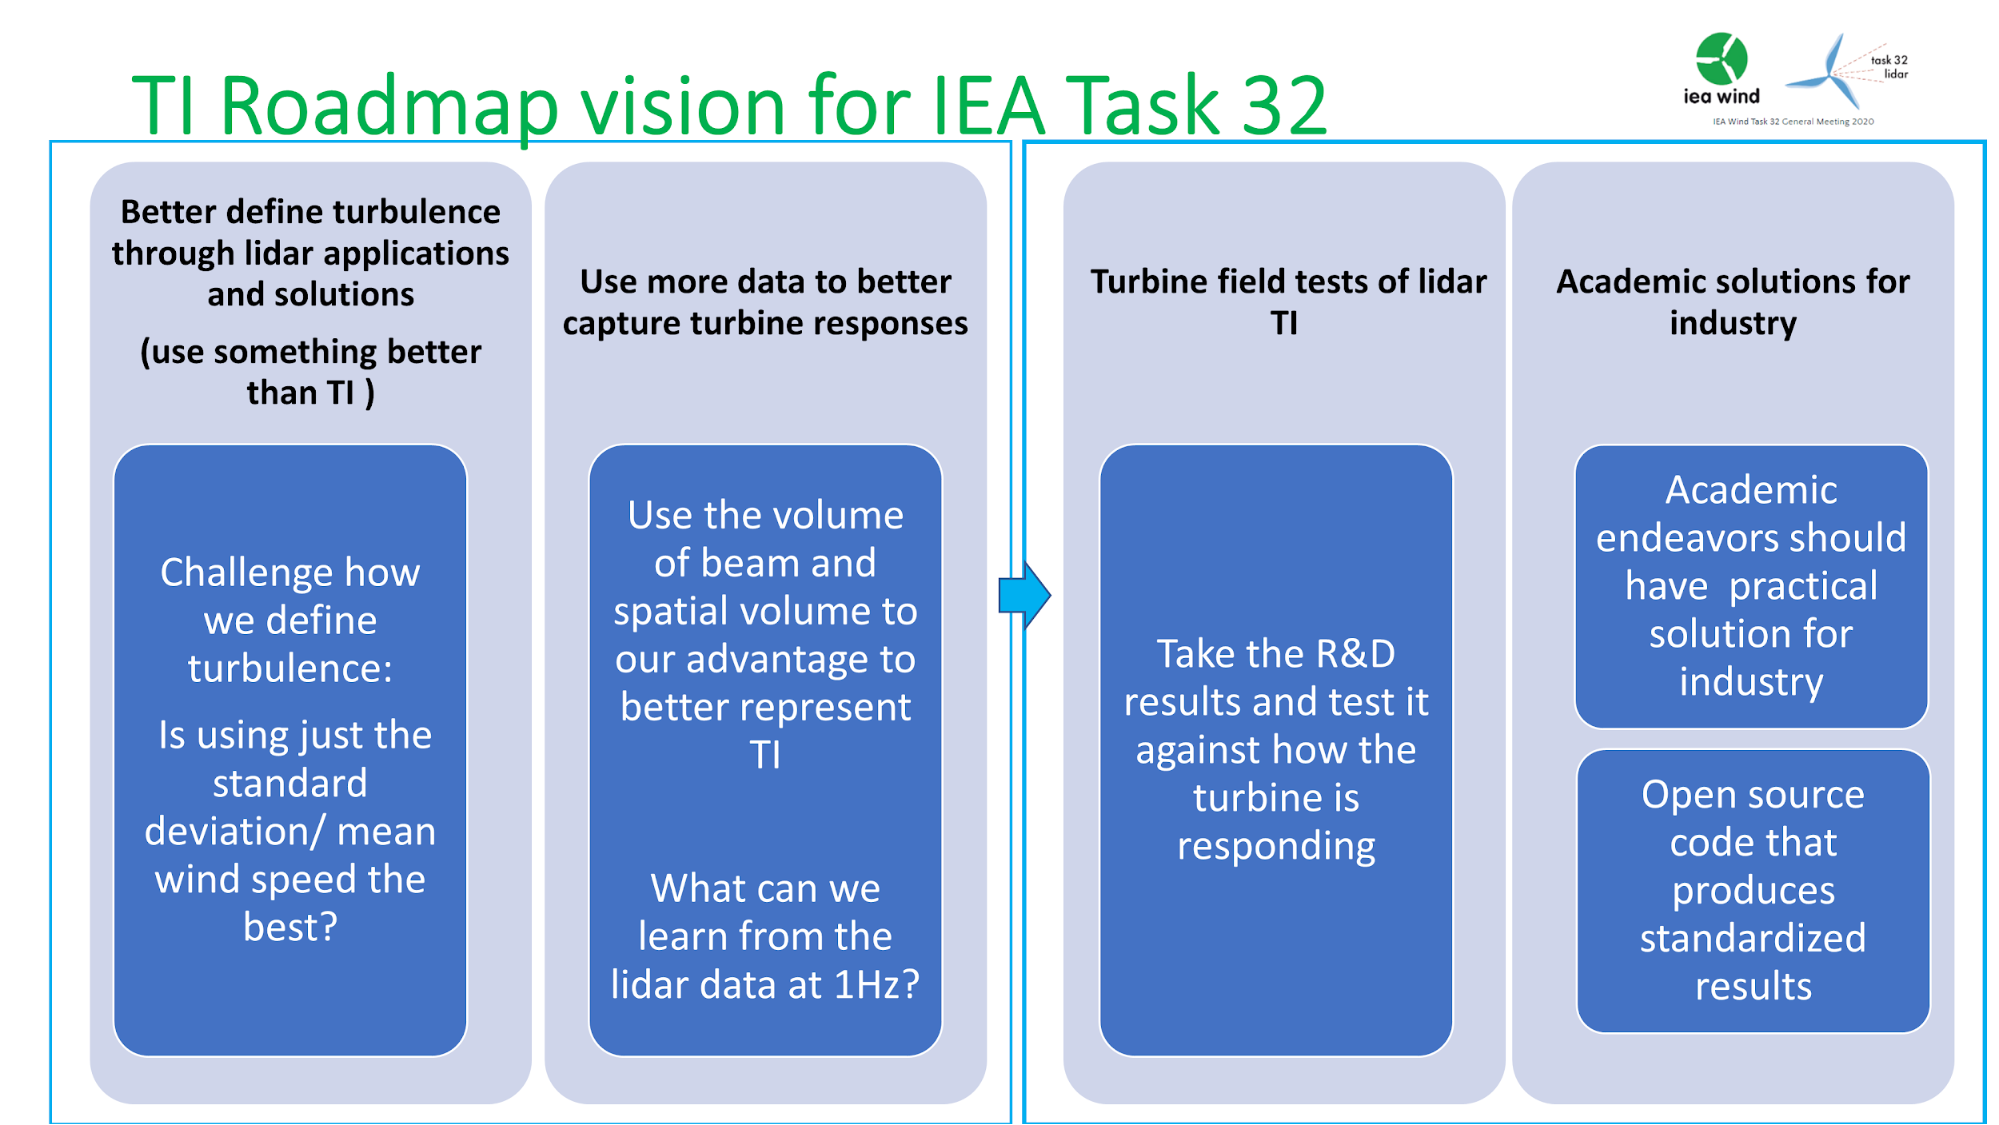
\includegraphics[width=0.85\textwidth]{figures/day3-Ti-group.png}
    }
    \caption{A lidar-derived turbulence data roadmap vision for Task 32 }
    \label{fig:day3-Ti-group}
\end{figure*}

\begin{figure*}[p]
    \centering
    \fbox{
    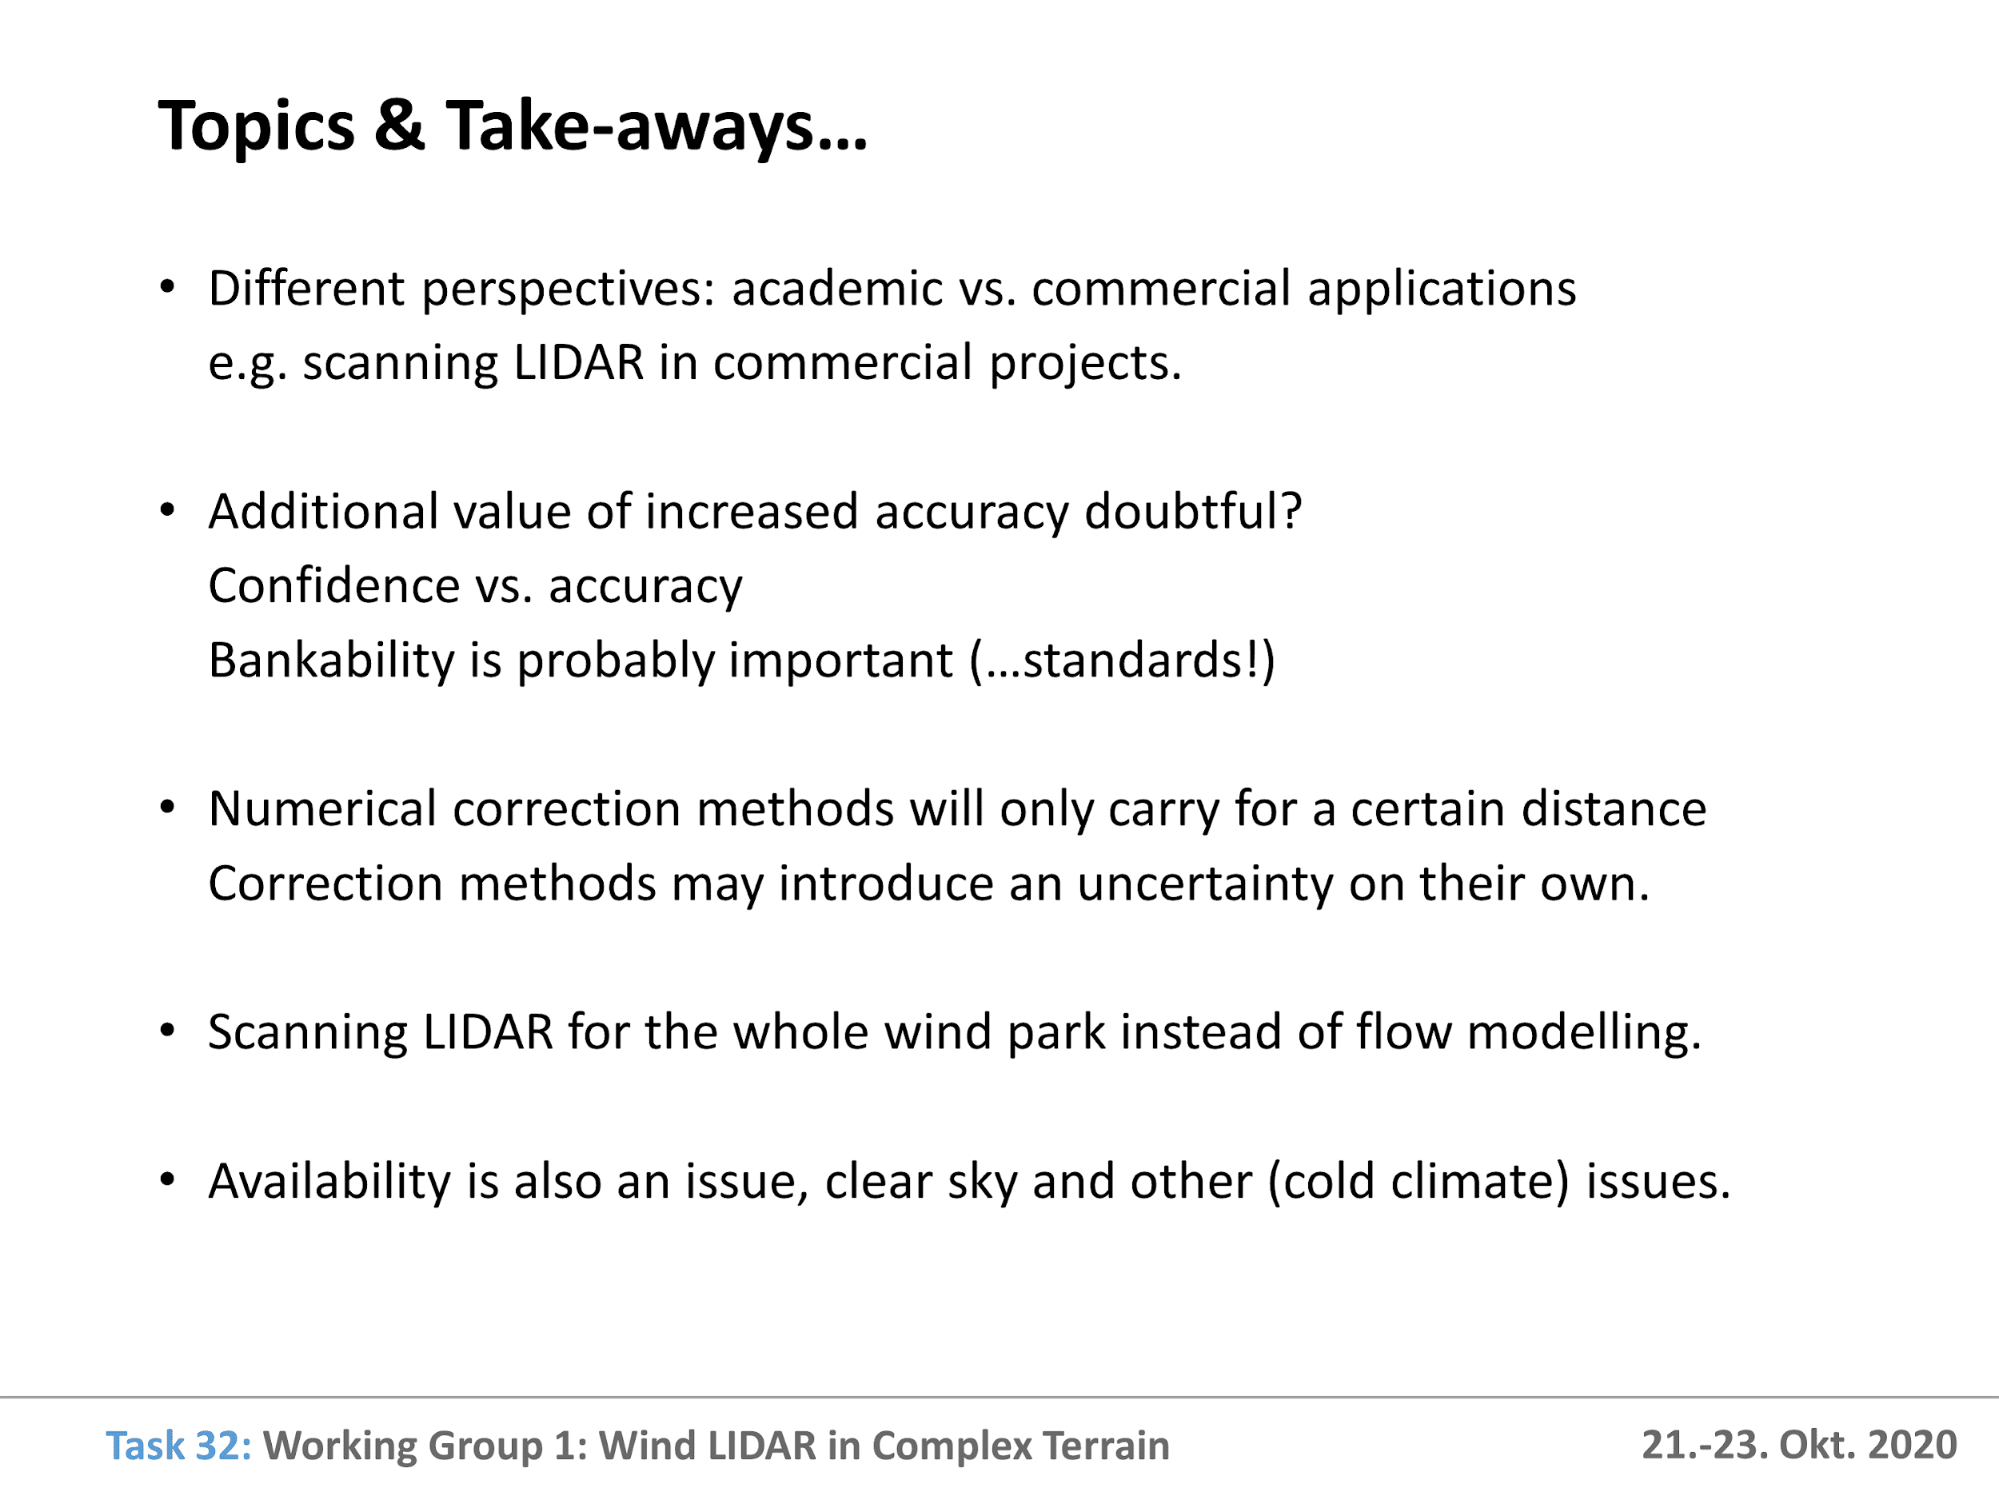
\includegraphics[width=0.85\textwidth]{figures/day3-complex-terrain.png}
    }
    \caption{Topics and take-aways from the complex terrain working session}
    \label{fig:day3-complex-terrain}
\end{figure*}

\begin{figure*}[p]
    \centering
    \fbox{
    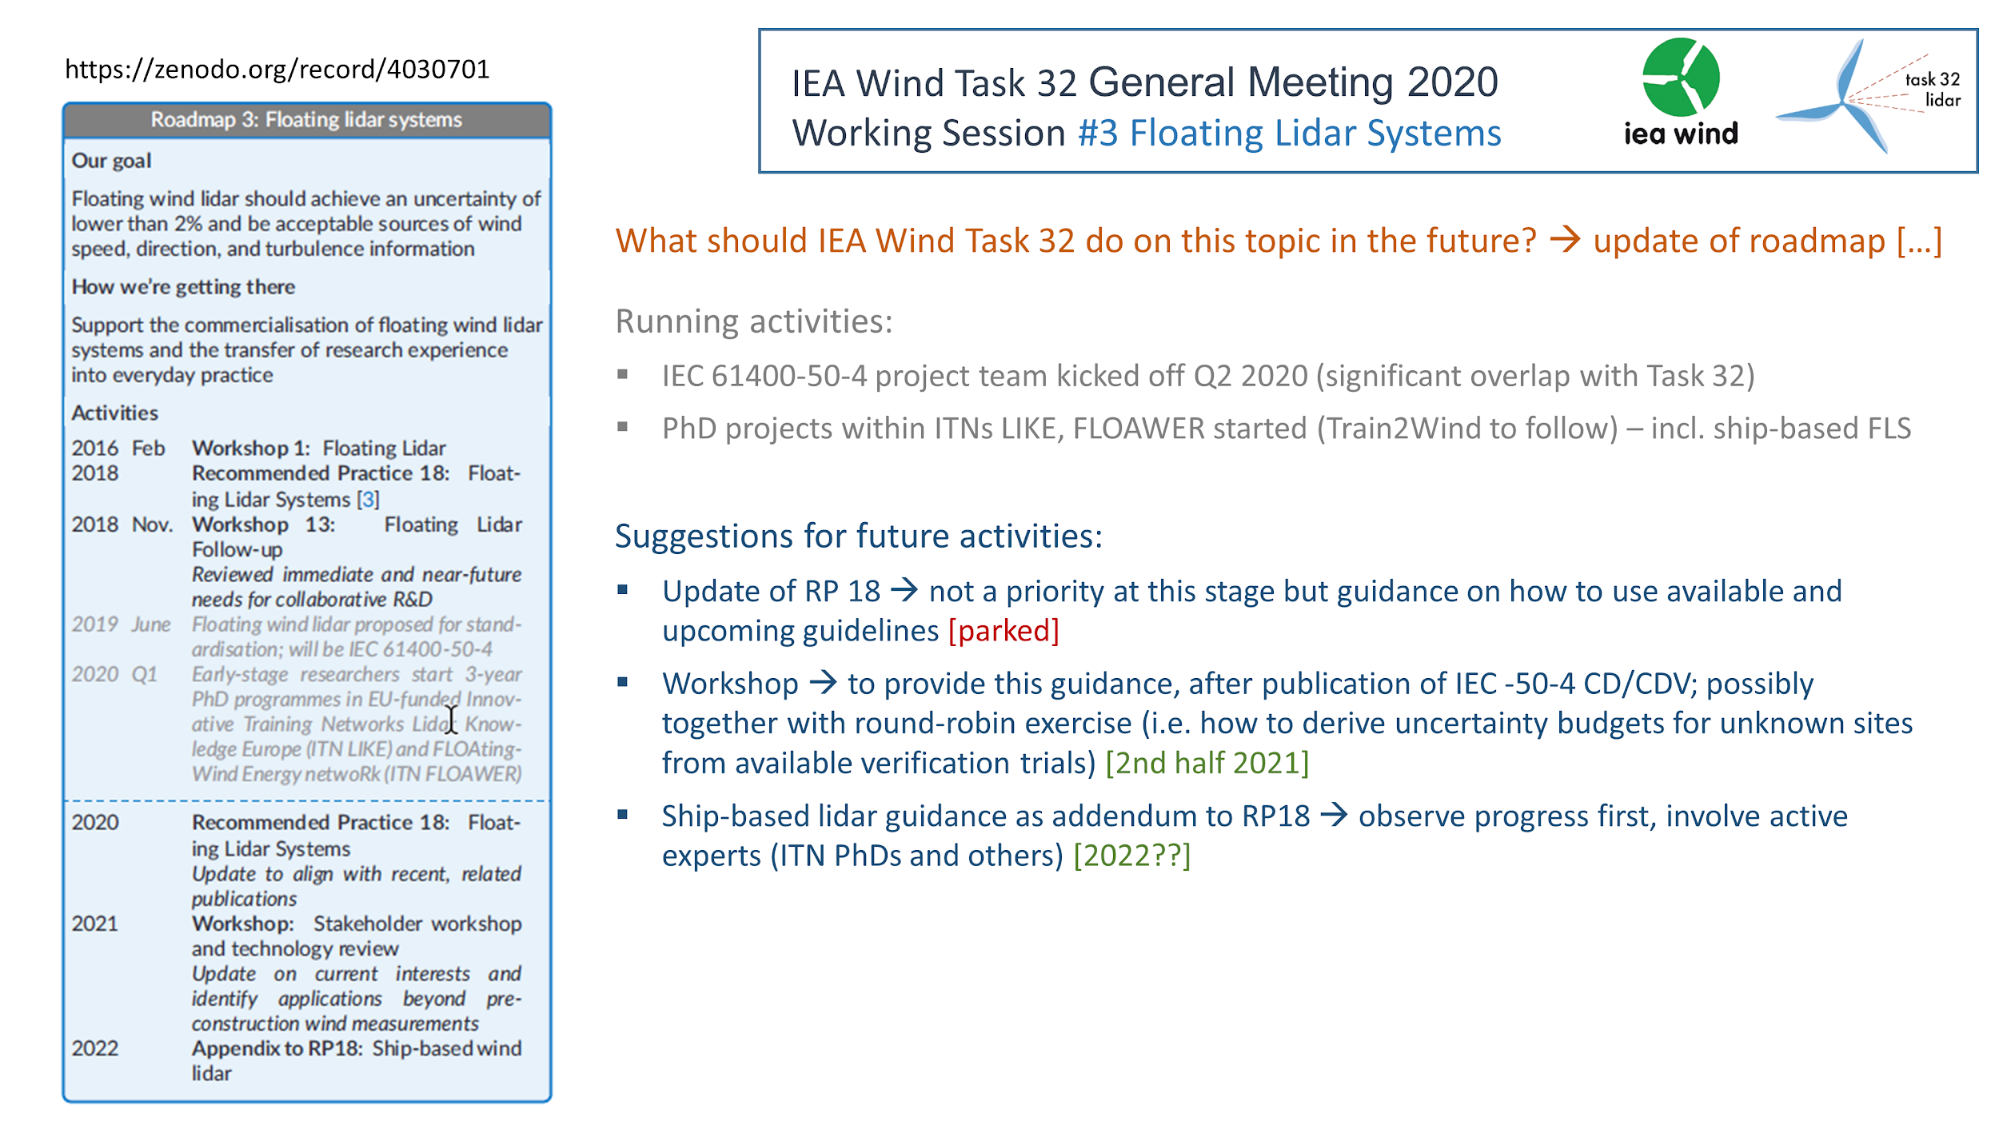
\includegraphics[width=0.85\textwidth]{figures/day3-floating-lidar.png}
    }
    \caption{Future activities for Task 32 around floating lidar systems.}
    \label{fig:day3-floating-lidar}
\end{figure*}

\begin{figure*}[p]
    \centering
    \fbox{
    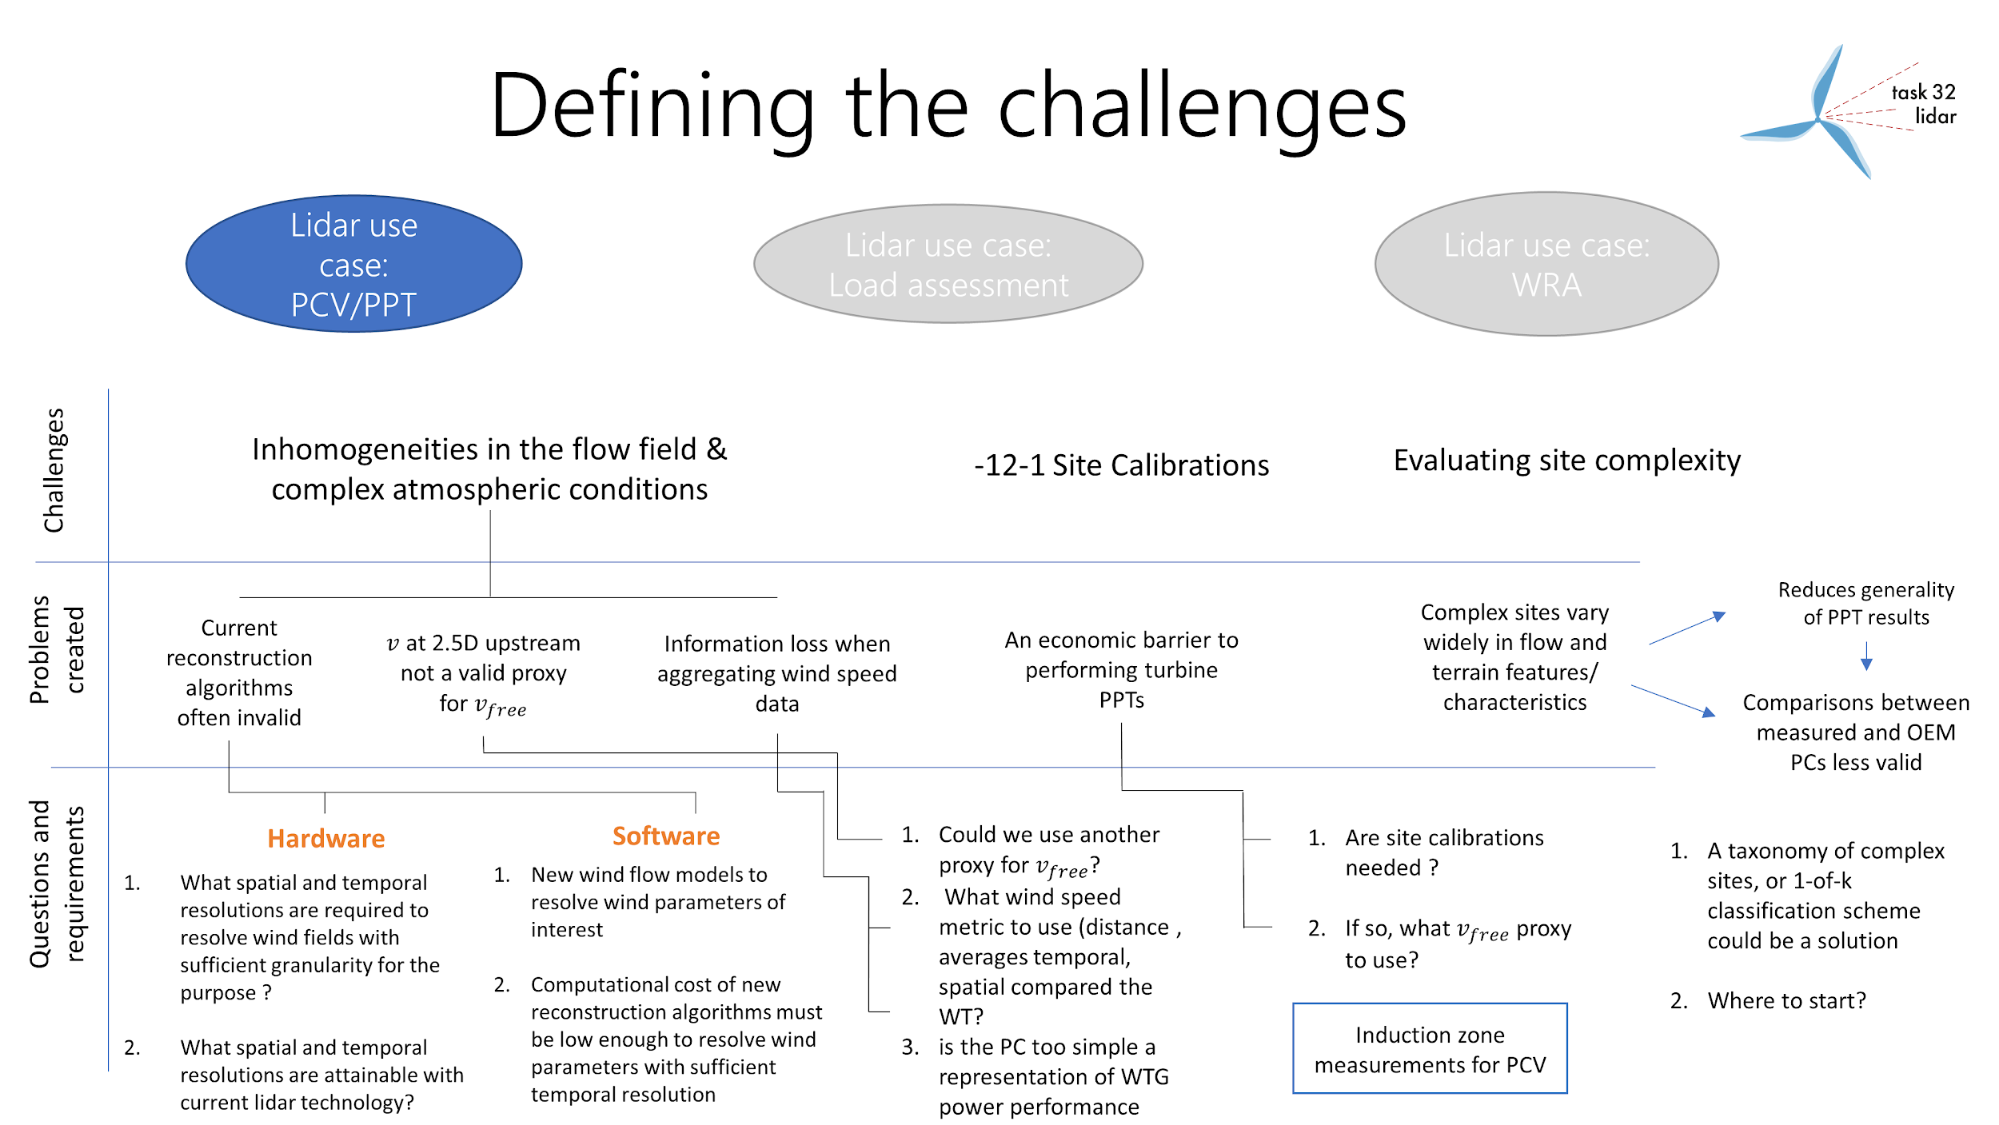
\includegraphics[width=0.85\textwidth]{figures/day3-nacelle-mounted.png}
    }
    \caption{Defining the challenge of using nacelle mounted lidar in complex terrain}
    \label{fig:day3-nacelle-mounted}
\end{figure*}

\begin{figure*}[p]
    \centering
    \fbox{
    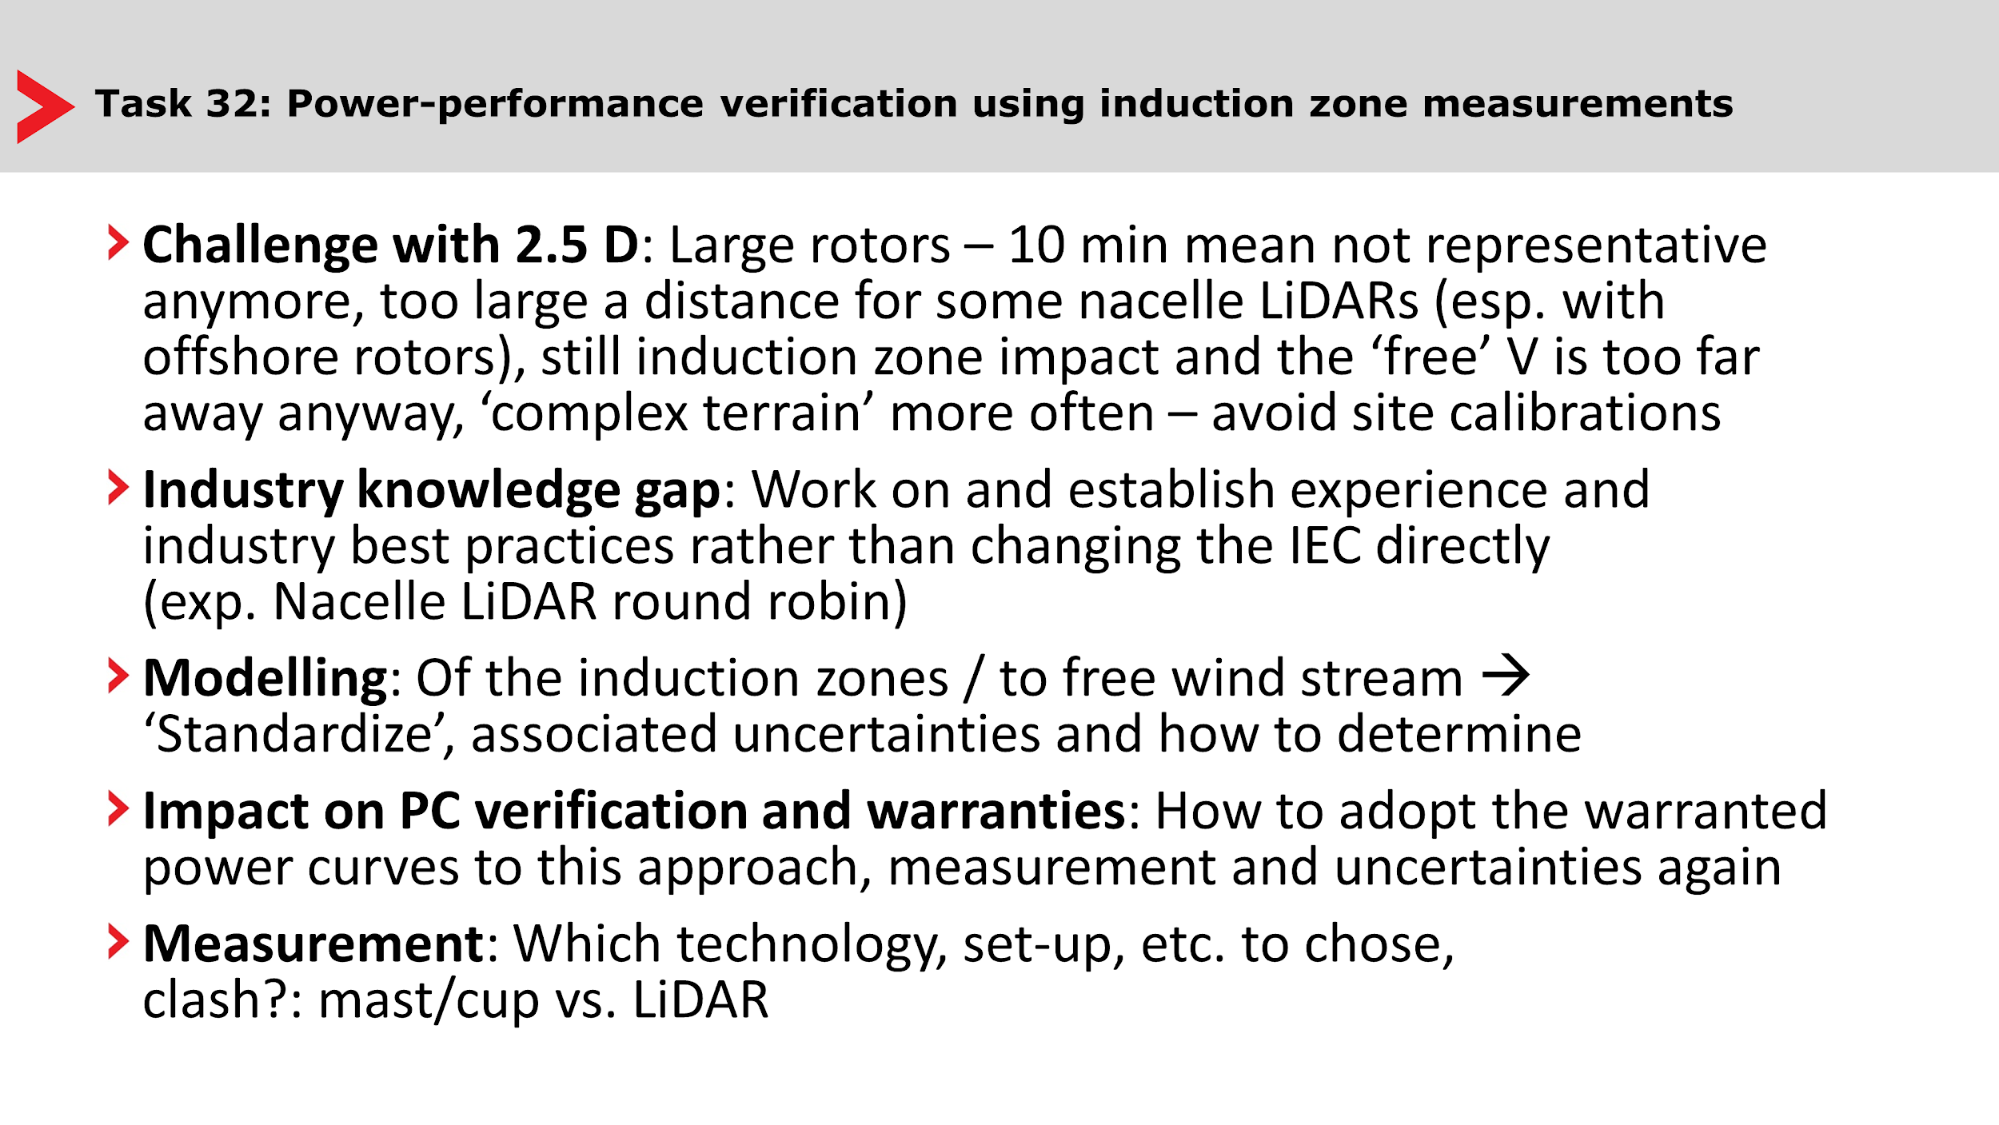
\includegraphics[width=0.85\textwidth]{figures/day3-powerperformance.png}
    }
    \caption{Opportunities and challenges with using measurements in the induction zone for power performance testing}
    \label{fig:day3-powerperformance}
\end{figure*}

\begin{figure*}[p]
    \centering
    \fbox{
    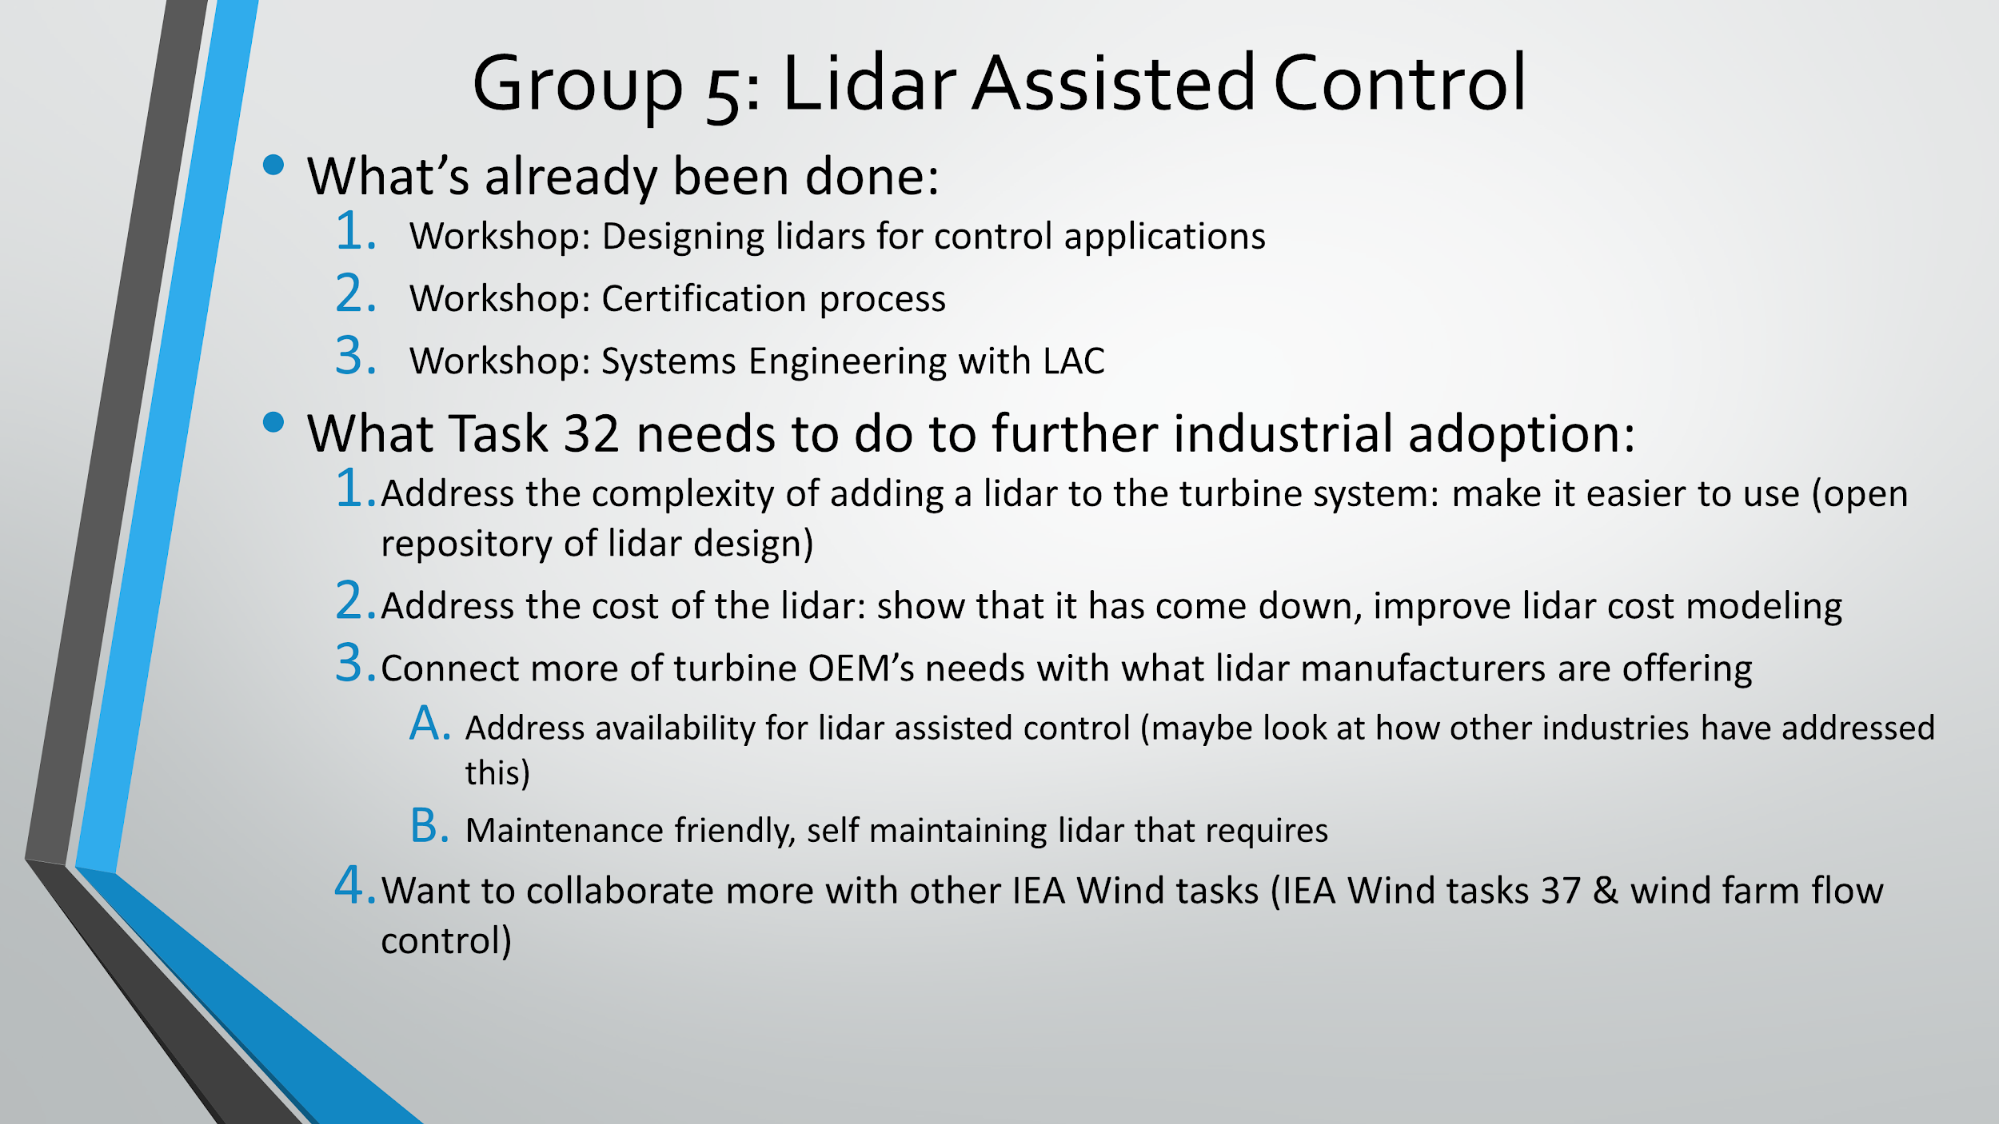
\includegraphics[width=0.85\textwidth]{figures/day3-LAC.png}
    }
    \caption{How Task 32 can enable adoption of lidar-assisted control of wind turbines and plants}
    \label{fig:day3-LAC}
\end{figure*}